\documentclass[10pt]{article}
\usepackage[margin=0.85in]{geometry}
\usepackage{amsmath,booktabs,multirow,graphicx,hyperref}
\setlength{\tabcolsep}{4pt}
\title{Weather-Conditioned Tropical Outage Prediction\\\large Development Experiment Report}
\author{}
\date{September 27, 2026}
\begin{document}\maketitle
\noindent\textbf{Status.} Completed development evaluation; not an independent confirmation or an operational weather-forecast test.
\section{Forecasting Results and Interpretation}

The complete campaign comprises 70 neural fits and 75 tree fits. Each of the 1,633 county--event pairs is evaluated exactly once in an outer event fold. All results below use the fixed public development panel; the sealed confirmation outcomes were not accessed.

\begin{table}[ht]\centering\small

\caption{Full 144-hour trajectory accuracy: design-weighted pooled metrics.}

\begin{tabular}{lrr}\toprule Model & MAE & RMSE \\\midrule

Zero forecast & 0.00978 & 0.05805 \\

Persistence & 0.00973 & 0.05728 \\

Damped persistence & 0.00971 & 0.05729 \\

Matched AsymODE host & 0.01078 & 0.04858 \\

Joint GCRK-rate model & 0.01171 & 0.05073 \\

ERA5 residual tree & 0.01439 & 0.05345 \\

Dual-weather residual tree & 0.01197 & 0.04813 \\

Dual-weather MAE tree & 0.00954 & 0.04921 \\

Inner-selected ensemble & 0.01108 & 0.04584 \\

\bottomrule\end{tabular}\end{table}

The inner-selected ensemble changes pooled RMSE relative to the matched host by -5.65\% (negative is better), with a paired family-bootstrap 95\% interval [-17.02\%, +4.24\%]. It improves RMSE on 10 of 15 systems. The corresponding MAE change is +2.81\%.

The joint GCRK-rate predictor changes RMSE relative to the matched host by +4.41\%, with a 95\% interval [+1.18\%, +9.46\%]. Because this arm changes the kernel and rate heads together, this is not an isolated test of geographic information.

The ensemble comparison does not establish a reliably positive gain at the stated interval level. Any favorable point estimate must therefore be interpreted as exploratory.

Against zero prediction, the ensemble reduces pooled RMSE by 21.03\% (95\% interval [10.85\%, 31.29\%]), but improves only 6 of 15 systems. Its RMSE reduction over the dual-weather residual tree is 4.75\% (interval [-2.11\%, 12.53\%]).

The lowest full-path MAE belongs to the dual-weather absolute-loss tree (0.00954); its MAE reduction relative to the host is 11.51\% (interval [3.57\%, 27.68\%]). Thus the RMSE-oriented ensemble and the absolute-loss tree represent different error tradeoffs. The present joint GCRK-rate arm does not support replacing the matched host.

\clearpage
\begin{table}[!ht]
\centering\small
\caption{Development event-held-out accuracy on 15 tropical systems. Design-weighted pooled MAE and RMSE of the public outage fraction; lower is better. Weather inputs are conditional hindcast information.}
\label{tab:tropical_forecasts}
\begin{tabular}{lcccccccc}
\toprule
\multirow{2}{*}{Model} & \multicolumn{4}{c}{MAE} & \multicolumn{4}{c}{RMSE} \\
\cmidrule(lr){2-5}\cmidrule(lr){6-9}
& $+1$ h & $+6$ h & $+24$ h & $+48$ h & $+1$ h & $+6$ h & $+24$ h & $+48$ h \\
\midrule
Zero forecast & 0.00088 & 0.00093 & 0.00993 & 0.01524 & 0.01588 & 0.01641 & 0.05660 & 0.07640 \\
Persistence & 0.00016 & 0.00029 & 0.00949 & 0.01498 & 0.00114 & 0.00187 & 0.05460 & 0.07539 \\
Damped persistence & 0.00016 & 0.00029 & 0.00948 & 0.01497 & 0.00114 & 0.00187 & 0.05460 & 0.07540 \\
Matched AsymODE host & 0.00053 & 0.00146 & 0.00921 & 0.01559 & 0.00512 & 0.01447 & 0.04026 & 0.05885 \\
Joint GCRK-rate model & 0.00051 & 0.00161 & 0.00969 & 0.01704 & 0.00415 & 0.01355 & 0.04216 & 0.06407 \\
ERA5 residual tree & 0.00145 & 0.00156 & 0.01025 & 0.02443 & 0.00686 & 0.00691 & 0.04490 & 0.07486 \\
Dual-weather residual tree & 0.00099 & 0.00105 & 0.00936 & 0.01924 & 0.00436 & 0.00455 & 0.04182 & 0.06625 \\
Dual-weather MAE tree & 0.00165 & 0.00169 & 0.00802 & 0.01514 & 0.01779 & 0.01816 & 0.04190 & 0.06249 \\
Inner-selected ensemble & 0.00099 & 0.00136 & 0.00860 & 0.01761 & 0.00573 & 0.01019 & 0.03744 & 0.06135 \\
\bottomrule
\end{tabular}
\end{table}

The four horizons are point predictions from the same 144-hour path; weights do not vary by horizon. The full-path RMSE ordering need not hold at every lead time. Persistence is particularly strong at the earliest leads in this panel. All seed, per-system and weighting-sensitivity results accompany the report.
\section{Methods}
\subsection{Tropical-cyclone forecast setting}
We study weather-conditioned county-level outage forecasting on the tropical
development subset of the public data panel. The subset contains 15 weather
systems and 1,633 county--event pairs, including weak systems with little or no
reported outage. For each system, a fixed forecast origin separates 72 hours
of historical outage observations from a 144-hour forecast window. The target
is the public outage fraction constructed by the data pipeline. We retain the
pipeline's observation masks, county sampling probabilities and design weights.
The historical information boundary is enforced on all outage-derived inputs.

The weather inputs comprise the available ERA5 and HRRR hazard summaries.
Missing weather hours have explicit availability indicators and retain the
upstream missing-value convention. Weather availability does not alter the
outage scoring mask. Physical county descriptors include terrain, vegetation,
soil and coastal-distance variables; six county background variables provide
electricity-service and population context. Imputation and standardization
are fitted separately within each training set. The 2023 interruption indices
are excluded from model inputs. Other static fields and customer denominators
retain the public panel's snapshot vintages.

\subsection{Predictors and joint training}
Our matched AsymODE reference uses the repository's two-rate outage-stock
model, with damage and recovery networks of widths 32 and 16, respectively.
The stock is advanced hourly by
\begin{equation}
 p_{i,t}=\operatorname{clip}_{[0,1]}
 \left[p_{i,t-1}+u_{i,t}(1-p_{i,t-1})-r_{i,t}p_{i,t-1}\right],
\end{equation}
initialized at the last observed outage fraction. Both neural predictors use
identical weather, historical-outage summary and county-context inputs.
The joint predictor additionally introduces the repository's geography-
conditioned response kernel and residual damage/recovery heads, each with
16 hidden units. The residual heads have zero initial output, and the kernel
opens gradually; the two predictors therefore have identical predictions at
initialization. All parameters are jointly optimized from scratch.
This comparison evaluates the combined prediction design, rather than
isolating the contribution of geography alone.

Every neural fit uses 900 Adam updates with batches of 128 county--event
pairs. Learning rates are 0.003 for damage/kernel parameters and 0.0003 for
recovery parameters, with gradient-norm clipping at one. Kernel calibration
statistics are refreshed on a fixed training-only sample. The final neural
predictions average seeds 0, 1 and 2. These models use reconstructed hazard
inputs and minibatch training, so they are distinct from the earlier
all-regime HOST experiment.

We also fit gradient-boosted trees to the entire forecast trajectory using
lead time as an input. Two residual models use squared-error loss and either
ERA5 alone or both weather sources; a direct model uses absolute-error loss.
Residuals are defined relative to exponential-decay persistence, whose
single decay parameter is fitted on the relevant training set. Tree settings
are fixed at 300 estimators, 15 leaves, learning rate 0.035 and a minimum of
80 samples per leaf. Zero and persistence predictors are reported alongside
the learned models.

\subsection{Event-held-out evaluation and ensemble selection}
We inherit the panel's five outer event folds without modification. Systems
belonging to a linked event group remain together. Inside each outer training
set, the four remaining event folds provide inner out-of-fold forecasts.
A single vector of nonnegative ensemble weights, summing to one, minimizes
the pooled design-weighted inner squared error. These weights remain fixed
across all 144 forecast hours. No outer outcome is used to select a weight,
checkpoint, seed or candidate configuration. Inner neural fits use seed zero;
final refits average three seeds, an approximation whose variance difference
is retained as a limitation.

For prediction $\widehat y_{i,t}$, target $y_{i,t}$, observation indicator
$m_{i,t}$ and county--event design weight $w_i$, we report
\begin{align}
 \mathrm{RMSE}&=\sqrt{\frac{\sum_{i,t}w_i m_{i,t}
 (\widehat y_{i,t}-y_{i,t})^2}{\sum_{i,t}w_i m_{i,t}}},\\
 \mathrm{MAE}&=\frac{\sum_{i,t}w_i m_{i,t}
 |\widehat y_{i,t}-y_{i,t}|}{\sum_{i,t}w_i m_{i,t}}.
\end{align}
Errors are pooled before taking the square root; fold RMSEs are not averaged.
We report the full-path metrics, individual point horizons, per-system and
exposure-stratum results, and untrimmed-weight and unweighted sensitivities.
Paired uncertainty intervals resample the 15 event families 2,000 times with
the saved outer predictions fixed. They do not capture repeated model
development or refitting uncertainty.

\paragraph{Scope of inference.}
This is event-held-out development evidence: the same county may occur in
other training storms, and prior development results informed the decision
to focus on tropical systems. The sealed confirmation tranche remains unread.
Future ERA5 and rolling HRRR fields provide conditional hindcast information,
not archived forecasts all issued at the outage forecast origin. Static
snapshots can also postdate historical storms. The experiment therefore does
not establish operational forecasting accuracy or independently confirmed
generalization.

\clearpage
\begin{figure}[p]\centering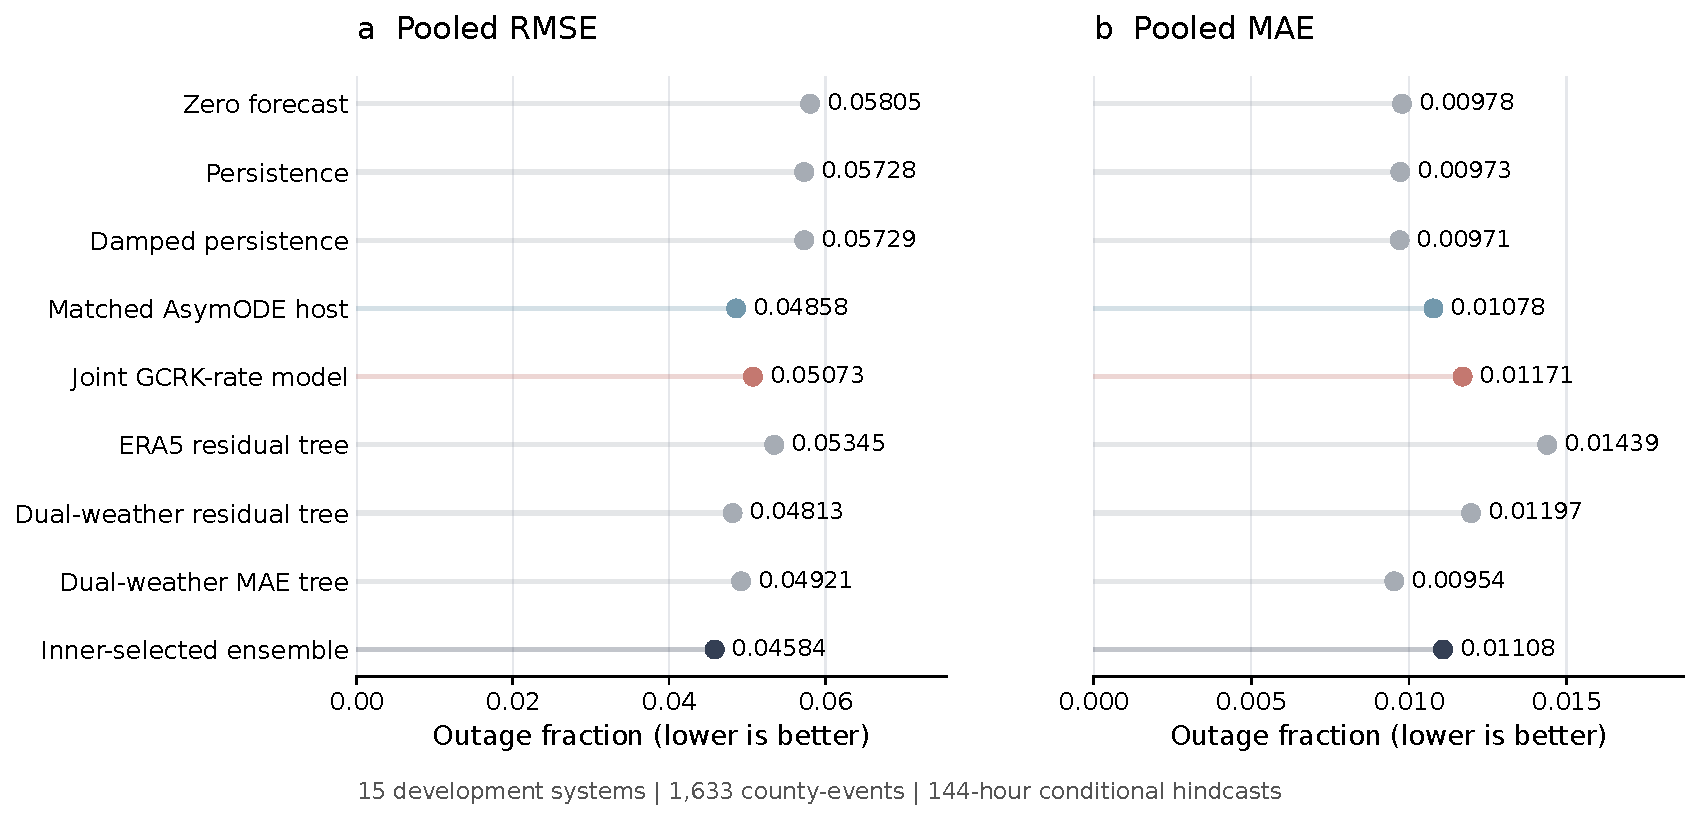
\includegraphics[width=\textwidth]{figures/forecast_metrics.pdf}
\caption{Full-path errors for all fixed candidates. The ensemble weights were selected only from inner event-fold predictions.}
\end{figure}
\begin{figure}[p]\centering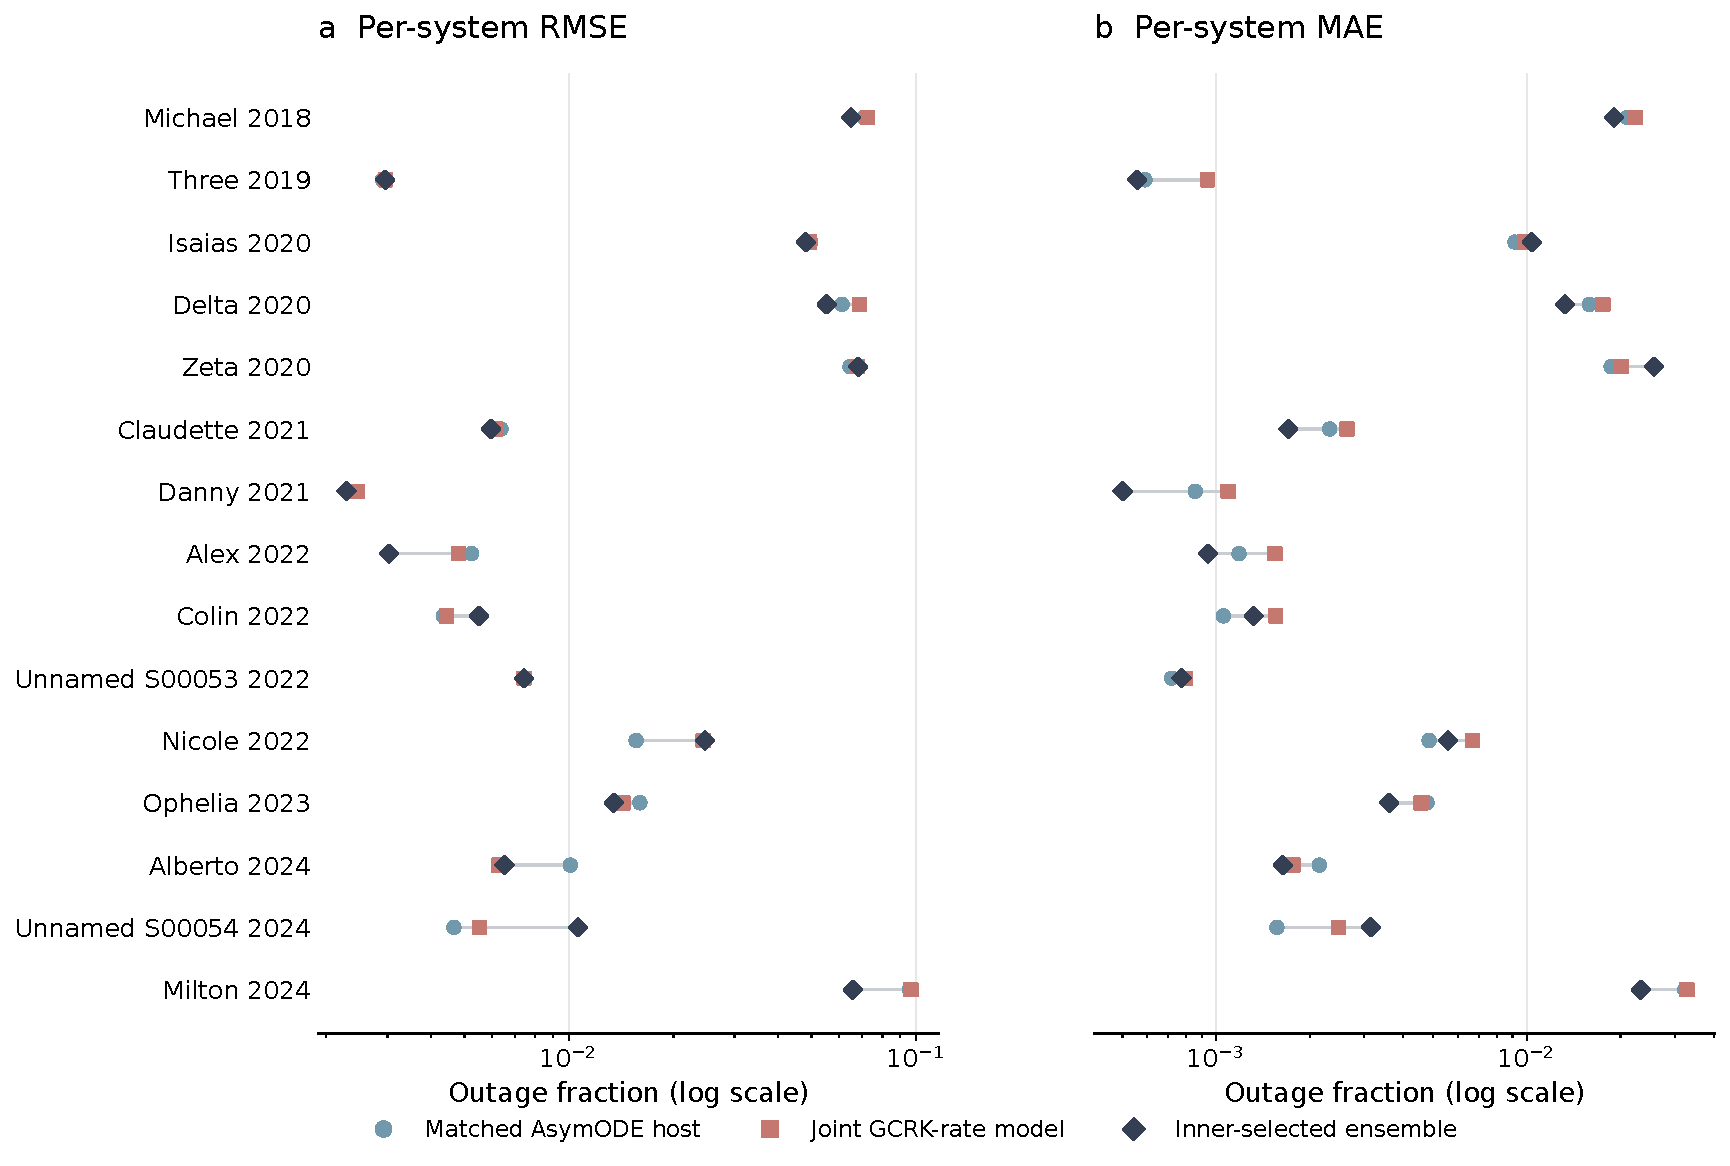
\includegraphics[width=\textwidth]{figures/storm_transfer.pdf}
\caption{Every tropical development system, including weak systems. Both horizontal axes use logarithmic scales.}
\end{figure}
\end{document}
